
%(BEGIN_QUESTION)
% Copyright 2009, Tony R. Kuphaldt, released under the Creative Commons Attribution License (v 1.0)
% This means you may do almost anything with this work of mine, so long as you give me proper credit

An instrument technician needs to connect two 4-20 mA transmitters to two analog inputs of a control system, the loop-powered transmitter to channel 01 and the line-powered (AC-powered) transmitter to channel 03.  All analog inputs on this system are configured for a maximum range of 0 to 3.5 volts DC:

$$\includegraphics[width=15.5cm]{i03851x01.eps}$$

Sketch the necessary wire connections, power sources, and other components (with necessary values) to make the circuit complete, so the control system will be able to monitor these two process variables.

\underbar{file i03851}
%(END_QUESTION)





%(BEGIN_ANSWER)

{\it Half credit for each working loop.  Any wiring errors resulting in a non-functioning loop preclude credit for that loop (i.e. no partial credit for wiring errors in each of the two loops).  Half-credit for answers not specifying resistor values.}

$$\includegraphics[width=15.5cm]{i03851x02.eps}$$

%(END_ANSWER)





%(BEGIN_NOTES)


{\bf This question is intended for exams only and not worksheets!}

%(END_NOTES)


